%% IEEE ICA 2026 -- Conference paper (IEEEtran, two-column).
%% Compile on Overleaf with pdfLaTeX + BibTeX (recompile twice; Overleaf is automatic).
%% Bibliography lives in the separate file references.bib.
%% Target length: 6 pages (see README.md for exact page-fitting levers).
\documentclass[conference]{IEEEtran}
\IEEEoverridecommandlockouts

\usepackage{cite}
\usepackage{amsmath,amssymb,amsfonts}
\usepackage{amsthm}
\usepackage{graphicx}
\usepackage{textcomp}
\usepackage{xcolor}
\usepackage{booktabs}
\usepackage{tikz}
\usetikzlibrary{arrows.meta,positioning,calc}
\usepackage[bookmarks=false]{hyperref}

\definecolor{slate}{HTML}{3E5C76}
\definecolor{clay}{HTML}{B07D48}
\definecolor{brick}{HTML}{9C4A3C}
\definecolor{hair}{HTML}{DED8CB}

% --- Review highlighting ----------------------------------------------------
% Every passage changed in the camera-ready revision is wrapped in \chg{...}.
% Compile as-is to see the changes in blue; set \reviewfalse (below) for the
% final clean submission -- \chg then prints its argument with no color.
\newif\ifreview\reviewtrue
\newcommand{\chg}[1]{\ifreview{\color{blue}#1}\else#1\fi}
% Blind-submission PDF metadata: force an empty Author field.
\hypersetup{pdfauthor={},pdftitle={Weight-Norm Growth and Update Geometry in Loss of Plasticity}}

\newtheorem{proposition}{Proposition}
\newtheorem{corollary}{Corollary}

\begin{document}

\title{Weight-Norm Growth and Update Geometry in\\
Loss of Plasticity:\\
A Matched-Step-Size Study}

\author{\IEEEauthorblockN{{Anonymous Authors}}
\IEEEauthorblockA{{Affiliation withheld for double-blind review}}}

\maketitle

\begin{abstract}
Continual-learning networks lose \emph{plasticity}: their ability to fit new
tasks declines over a task stream. Prior accounts link this to update magnitude
(weight-norm growth, distance from initialization, dormant units), whereas subspace
methods constrain update direction. We ask whether direction alone preserves
plasticity when magnitude is fixed. Our control renormalizes each candidate update
to the Euclidean norm of the plain-SGD step at the same parameters, leaving only
direction to vary. On a $100$-task permuted-MNIST stream with a
$784$--$16$--$16$--$10$ MLP (five seeds), we report three findings.
(i)~Across seven update rules, final global parameter norm and plasticity decay are
strongly associated ($r{=}0.97$, $n{=}7$ arm means), and an L2-init strength sweep
moves both together; the association weakens at width $64$ ($r{=}0.45$) and is
absent where plasticity loss is mild (width $128$, rotated MNIST). (ii)~A simple
fixed-step identity shows that orthogonal steps raise the squared norm by exactly
$\eta^{2}$, while any norm reduction requires
$\langle\theta,d\rangle\le-\eta/2$. (iii)~A radial sweep confirms inward
steering lowers the norm monotonically, but its best setting ($0.763$ accuracy)
trails magnitude methods that reduce the norm (L2-init $0.819$, Shrink\&Perturb $0.799$),
while strong inward steering collapses learning. A targeted per-unit variant nearly
eliminates dormant units but does not improve accuracy. In this regime, magnitude
control preserves plasticity better than matched-step directional control.
\end{abstract}

\begin{IEEEkeywords}
continual learning, loss of plasticity, weight norm, update geometry, permuted
MNIST, matched-magnitude control
\end{IEEEkeywords}

\section{Introduction}
A network trained on a stream of tasks degrades in two distinct ways.
\emph{Catastrophic forgetting}~\cite{mccloskey1989,goodfellow2013}
is loss of performance on \emph{previously learned} tasks; \emph{loss of
plasticity}~\cite{dohare2024,lyle2023,abbas2023} is erosion of the capacity
to fit \emph{future} tasks---after many tasks, a network fits the next one worse
than it fit early ones, even when tasks are unrelated. This paper focuses on the
second phenomenon in a single, deliberately controlled setting.

\textbf{The question and gap.} Two accounts coexist: \emph{magnitude/capacity}
accounts tie rigidity to how far and how long weights move---weight-norm growth,
distance from initialization, dormant units, representation
collapse~\cite{ash2020,sokar2023,lyle2022,berariu2021,springer2025}---while
\emph{directional} methods constrain updates to
subspaces~\cite{lopezpaz2017,farajtabar2020,saha2021gpm,zeng2019owm,chaudhry2020orthog}
and curvature analyses relate landscape direction to
plasticity~\cite{lewandowski2023}. A standard optimizer changes direction and
magnitude together, entangling them. We ask: \emph{does update direction have an
independent plasticity-preserving effect when the update magnitude is held
fixed?} This comparison---direction varied at \emph{exactly} constant
magnitude---has not, to our knowledge, been isolated for \emph{future}-trainability;
existing directional methods target the \emph{past}~\cite{farajtabar2020,saha2021gpm}.

\textbf{Scope.} Our \emph{primary} regime is a controlled $100$-task permuted
MNIST~\cite{lecun1998} stream with a warm-started $784$--$16$--$16$--$10$ MLP,
matched update magnitude for directional interventions, the \emph{global}
Euclidean parameter norm, and five seeds. To map boundary conditions we add wider
MLPs (widths $64$, $128$) and a different task geometry (rotated MNIST, MLP and a
small CNN) {under the same protocol (CNN differences noted in Sec.~\ref{sec:setup})}. We do not claim
universality across architectures, normalization schemes, or optimizers.

\noindent\textbf{Contributions.}
\begin{itemize}
\item A reproducible matched-step permuted-MNIST regime---instrumented with global
parameter norm, unit-dormancy, and effective feature rank---in which plain SGD
loses plasticity, together with an empirical \emph{association} between
weight-norm growth and plasticity decay ($r{=}0.97$, $n{=}7$),
norm-control-strength sweep, and a five-regime test where the association
\emph{weakens with width and {is absent where plasticity loss is mild}} across
capacity and task geometry
(Secs.~\ref{sec:setup},~\ref{sec:results}).
\item A \emph{fixed-step, global-norm} {identity} (Prop.~\ref{prop:floor}) with two
corollaries and an explicit statement of what it does and does \emph{not}
establish
(Sec.~\ref{sec:theory}).
\item A radial-coefficient sweep (plus an orthogonal endpoint) showing the
geometry's norm/accuracy trade-off---no directional setting matches magnitude
control---with a magnitude-method comparison and an honest negative for the
targeted per-unit method
 (Sec.~\ref{sec:results}).
\end{itemize}

\noindent\textbf{Hypotheses.} We test whether \emph{(H1)} weight-norm growth
predicts plasticity decay; \emph{(H2)} fixed-magnitude directional steering
preserves plasticity; \emph{(H3)} direct magnitude control preserves plasticity;
and \emph{(H4)} the norm--plasticity relationship generalizes across width and
task regime. In the tested regimes, \textbf{H1} and \textbf{H3} {are} supported;
\textbf{H2} is \emph{not} supported as a competitive mechanism (a mild inward
bias only modestly beats SGD, no directional setting reaches magnitude control,
and strong inward steering collapses learning), and \textbf{H4} is \emph{not}
supported as a universal claim (the association weakens with width and {is
absent where plasticity loss is mild}); we write {``supported/not supported in
the tested regime'' rather than ``proved/disproved.''}

\section{Related Work}
\textbf{Catastrophic forgetting.} Interference in sequential
learning~\cite{mccloskey1989,goodfellow2013} is reduced by
regularizing key weights (EWC~\cite{kirkpatrick2017}, SI~\cite{zenke2017},
MAS~\cite{aljundi2018mas}), replay/distillation (LwF~\cite{li2017lwf},
iCaRL~\cite{rebuffi2017}, GEM/A-GEM~\cite{lopezpaz2017,chaudhry2019agem}), or
parameter isolation (HAT~\cite{serra2018hat}); surveys map out this
space~\cite{vandeven2019,parisi2019,delange2021}. These methods address the \emph{past}.

\textbf{Directional / subspace methods.} Orthogonal Gradient
Descent~\cite{farajtabar2020}, Gradient Projection Memory~\cite{saha2021gpm},
orthogonal weight modification~\cite{zeng2019owm}, and low-rank orthogonal
subspaces~\cite{chaudhry2020orthog} project updates to avoid disturbing prior
tasks---directional but \emph{past}-facing; none isolates a plasticity-preserving
directional effect at fixed magnitude for future tasks.

\textbf{Loss of plasticity.} Continual Backprop showed that standard optimizers
lose plasticity over long streams and that re-initializing low-utility units
restores it~\cite{dohare2024,dohare2021cbp}. Related analyses tie the effect to a
primacy bias~\cite{nikishin2022}, capacity loss~\cite{lyle2022},
representation-level effects~\cite{lyle2023}, dormant neurons~\cite{sokar2023}, and
deep RL~\cite{abbas2023}; plasticity injection~\cite{nikishin2023} and joint
forgetting/plasticity treatments~\cite{elsayed2024} have also been proposed. These
are broadly magnitude/capacity accounts. Lyle et al.~\cite{lyle2024disentangling}
show that plasticity loss has several distinct causes, including parameter-norm
growth as one.

\textbf{Magnitude, initialization, and training regime.} Warm-starting harms
generalization, while Shrink\&Perturb restores it~\cite{ash2020}; L2 regularization
toward initialization (L2-init) maintains plasticity by limiting weight-norm
growth~\cite{kumar2023}; overtraining increases fragility~\cite{springer2025}; and
training regime, critical periods, and initialization all shape
trainability~\cite{mirzadeh2020,achille2019,he2015,berariu2021,kingma2015adam}.
Curvature directions correlate with plasticity loss~\cite{lewandowski2023}, but
these analyses are retrospective and do not test update direction at fixed
magnitudes---exactly the controlled intervention we supply.

\section{Problem Formulation}\label{sec:formulation}
Let $\theta\in\mathbb{R}^{d}$ denote the global parameter vector. Plain SGD produces
$\Delta\theta=-\eta_0\nabla_\theta\mathcal{L}(\theta)$ with step size
$\eta=\lVert\Delta\theta\rVert$. We study rules $\theta\!\leftarrow\!\theta+\Delta\theta'$.
To isolate \emph{direction} from \emph{magnitude} we impose the
\emph{matched-step} control: at every step,
\begin{equation}
\lVert\Delta\theta'\rVert=\lVert\Delta\theta\rVert=\eta
\quad\text{(exact renormalization).}
\label{eq:matched}
\end{equation}
A \emph{directional intervention} is any $\Delta\theta'$ satisfying
\eqref{eq:matched} that differs from $\Delta\theta$ only in direction
$d=\Delta\theta'/\eta$, $\lVert d\rVert=1$. Unless stated otherwise,
$\lVert\theta\rVert$ denotes the \emph{global} Euclidean norm of the trainable
backbone parameters; this is distinct from per-layer or per-unit norms, a
distinction that matters in
 Sec.~\ref{sec:method}.

For a task stream ${T_1,\dots,T_K}$, let $a_t$ be the test accuracy on $T_t$
immediately after training on it---an \emph{operational} proxy for future-task
trainability, so a falling $a_t$ signals a diminishing ability to fit new tasks.
The \emph{plasticity decay} is
\begin{equation}
\mathrm{decay}=\max_t a_t-\frac{1}{|\mathcal{E}|}\sum_{t\in\mathcal{E}}a_t,
\quad \mathcal{E}=\text{last }10\%\text{ of tasks},
\label{eq:decay}
\end{equation}
reported as a fraction (e.g.\ decay $0.133$ denotes a $13.3$-point drop). This
peak-to-tail measure is less noisy than the final task alone, and late-task-mean and
area-under-curve summaries agree. We also log the global weight norm
$\lVert\theta\rVert$, the dormant-unit fraction (mean absolute activation
$<10^{-3}$ on a probe batch), and the stable (effective) rank of penultimate
features $\lVert F\rVert_F^{2}/\lVert F\rVert_2^{2}$.

\section{A Fixed-Step, Global-Norm Identity}\label{sec:theory}
The following elementary identity constrains how a \emph{fixed-length} update can
change the \emph{global} parameter norm.

\begin{proposition}[Fixed-step norm identity]\label{prop:floor}
Let $\theta\in\mathbb{R}^{d}$ and $\theta'=\theta+\eta d$ with $\lVert d\rVert=1$,
$\eta>0$. Then
\begin{equation}
\lVert\theta'\rVert^{2}=\lVert\theta\rVert^{2}+2\eta\langle\theta,d\rangle+\eta^{2}.
\label{eq:law}
\end{equation}
\end{proposition}
\begin{proof}
$\lVert\theta+\eta d\rVert^{2}
=\lVert\theta\rVert^{2}+2\eta\langle\theta,d\rangle+\eta^{2}\lVert d\rVert^{2}$,
and $\lVert d\rVert=1$.
\end{proof}

\begin{corollary}[Orthogonal steps raise the squared norm]\label{cor:orth}
If $\langle\theta,d\rangle=0$ then
$\lVert\theta'\rVert^{2}=\lVert\theta\rVert^{2}+\eta^{2}$: the \emph{squared}
global norm increases by exactly $\eta^{2}$, for every unit direction in
$\theta^{\perp}$. Hence a fixed-length step taken orthogonal to $\theta$ cannot
decrease the global norm.
\end{corollary}

\begin{corollary}[Reducing the global norm taxes the unit budget]\label{cor:inward}
$\lVert\theta'\rVert\le\lVert\theta\rVert$ holds iff
$\langle\theta,d\rangle\le-\eta/2$. Writing $\hat\theta=\theta/\lVert\theta\rVert$,
the inward radial component of $d$ then satisfies
$\langle d,-\hat\theta\rangle=-\langle\theta,d\rangle/\lVert\theta\rVert
\ge \eta/(2\lVert\theta\rVert)$. Because $\lVert d\rVert=1$, the portion of the
unit direction available for any other (e.g.\ descent) direction is at most
$\sqrt{1-\big(\eta/(2\lVert\theta\rVert)\big)^{2}}$ when
$\lVert\theta\rVert\ge\eta/2$. Thus at fixed step size, reducing the global norm
necessarily consumes part of the update's unit budget.
\end{corollary}

\noindent\textbf{Radial--tangential reading.} Decompose $d=d_{\parallel}+d_{\perp}$
with radial part
$d_{\parallel}=\big(\langle\theta,d\rangle/\lVert\theta\rVert^{2}\big)\theta$ and
$\langle\theta,d_{\perp}\rangle=0$. By~\eqref{eq:law} the first-order norm change
$\eta\langle\theta,d\rangle/\lVert\theta\rVert$ depends only on $d_{\parallel}$;
$d_{\perp}$ leaves $\lVert\theta\rVert$ unchanged to first order. Since
$\lVert d_{\parallel}\rVert^{2}+\lVert d_{\perp}\rVert^{2}=1$, spending more of the
unit budget on an inward radial component (to shrink the norm,
Cor.~\ref{cor:inward}) leaves less for the tangential/descent direction. The
minimum cost in Cor.~\ref{cor:inward} remains small when $\lVert\theta\rVert\gg\eta$:
simply holding the norm uses a fraction $\eta/(2\lVert\theta\rVert)$ of the budget.
Rapidly shrinking the norm requires a larger radial allocation;
Sec.~\ref{sec:results} measures what that allocation costs in accuracy. We present
this as a geometric interpretation, not a new optimization theorem.

\noindent\textbf{Scope of Prop.~\ref{prop:floor}.} {\emph{Proven:} for a fixed
global step, orthogonal steps raise the squared norm by $\eta^{2}$
(Cor.~\ref{cor:orth}), while any reduction requires
$\langle\theta,d\rangle\le-\eta/2$, i.e., an inward component of at least
$\eta/(2\lVert\theta\rVert)$ (Cor.~\ref{cor:inward}; Fig.~\ref{fig:geom}).}
\emph{Not covered:}
per-layer/per-unit norms, adaptive or per-coordinate steps, normalization layers
(which rescale activations independently of $\lVert\theta\rVert$), and pathologies
not mediated by global-norm growth. Thus, it does \emph{not} imply that every
directional or geometric method must fail---only that fixed-step, global-norm
directional interventions are so constrained.

\begin{figure}[tb]
\centering
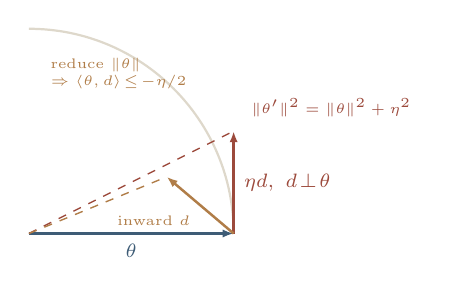
\begin{tikzpicture}[font=\scriptsize,scale=1.0]
\coordinate (O) at (0,0);
\coordinate (T) at (2.6,0);
\draw[draw=hair,line width=0.8pt] (2.6,0) arc[start angle=0,end angle=90,radius=2.6];
\draw[-{Latex[length=1.4mm]},slate,line width=0.9pt] (O) -- (T) node[midway,below]{$\theta$};
\coordinate (Torth) at (2.6,1.3);
\draw[-{Latex[length=1.4mm]},brick,line width=0.9pt] (T) -- (Torth) node[midway,right]{$\eta d,\ d\!\perp\!\theta$};
\draw[draw=brick,dashed,line width=0.5pt] (O) -- (Torth);
\node[brick,anchor=west,font=\tiny] at (2.7,1.6) {$\lVert\theta'\rVert^{2}=\lVert\theta\rVert^{2}+\eta^{2}$};
\coordinate (Tin) at (1.75,0.72);
\draw[-{Latex[length=1.4mm]},clay,line width=0.9pt] (T) -- (Tin) node[midway,below left,font=\tiny]{inward $d$};
\draw[draw=clay,dashed,line width=0.5pt] (O) -- (Tin);
\node[clay,anchor=north west,align=left,font=\tiny] at (0.15,2.35)
  {reduce $\lVert\theta\rVert$\\$\Rightarrow\langle\theta,d\rangle\!\le\!-\eta/2$};
\end{tikzpicture}
\caption{{Geometry of Prop.~\ref{prop:floor}. A fixed-length step orthogonal to
$\theta$ (brick) moves \emph{outside} the current norm sphere, raising the squared
norm by exactly $\eta^{2}$ (Cor.~\ref{cor:orth}). Landing \emph{inside} (clay)
requires $\langle\theta,d\rangle\le-\eta/2$, i.e., an inward radial component of at
least $\eta/(2\lVert\theta\rVert)$ of the unit direction (Cor.~\ref{cor:inward}).}}
\label{fig:geom}
\end{figure}

\section{Update Rules and Ablations}\label{sec:method}
All rules below obey~\eqref{eq:matched} where indicated. Given the SGD step
$\Delta\theta$ and radial unit vector $\hat\theta=\theta/\lVert\theta\rVert$:

\textbf{Directional ablations (matched step, global norm).} \emph{Orthogonal
steering} removes the radial component,
$\Delta\theta'\propto\Delta\theta-(\Delta\theta^{\top}\hat\theta)\,\hat\theta$;
\emph{inward steering} adds a $-\hat\theta$ bias,
$\Delta\theta'\propto\Delta\theta-\gamma\eta\,\hat\theta$ {(Table~\ref{tab:main}
uses $\gamma{=}0.6$)}; both are renormalized
to $\eta$, realizing the two regimes of Cor.~\ref{cor:orth}--\ref{cor:inward}.
These arms are deliberately \emph{diagnostic} interventions that isolate the
proposition's geometric regimes (Sec.~\ref{sec:results} extends the inward endpoint
into a full radial sweep), not proposed algorithms; existing subspace methods
(OGD~\cite{farajtabar2020}, GPM~\cite{saha2021gpm}, OWM~\cite{zeng2019owm}) instead
reduce interference with \emph{past} tasks---a different objective.

\textbf{Adaptive-Norm-Revive (ANR): a separate per-unit hypothesis.} ANR tests
whether \emph{targeted, per-unit} magnitude control beats global shrinking---an
independent question, outside Prop.~\ref{prop:floor}, which concerns the
\emph{global} norm. Between tasks it (i) rescales only hidden units whose per-unit
incoming-weight norm exceeds a target $\tau{=}3.0$, and (ii) re-initializes
(Kaiming~\cite{he2015}) only units with mean absolute activation $<10^{-3}$ on a probe batch,
zeroing their outgoing weights so revival does not perturb the current mapping. Both
hyperparameters are \emph{fixed a priori}. A component ablation
(Sec.~\ref{sec:results}) separates its two mechanisms.

\textbf{Reference baselines.} Plain SGD; L2-init~\cite{kumar2023}
($\lambda{=}10^{-2}$); Shrink\&Perturb~\cite{ash2020} ($s{=}0.7,\sigma{=}0.01$);
and Continual Backprop~\cite{dohare2024} (utility-based unit resets). L2-init and
Shrink\&Perturb are \emph{magnitude} methods: they are permitted to change $\eta$
and thereby reduce $\lVert\theta\rVert$, and are not bound by
Prop.~\ref{prop:floor}. We refer to these as \emph{reference magnitude methods}
rather than state of the art.


\section{Experimental Setup}\label{sec:setup}
{We use permuted MNIST~\cite{goodfellow2013,lecun1998}: each task applies a fixed
random pixel permutation while labels remain unchanged, so a shared $10$-way head isolates
sequential adaptation without class-incremental confounds. The backbone is a
$784$--$16$--$16$--$10$ ReLU MLP, warm-started by carrying its weights across task
boundaries without reinitialization (standard random initialization precedes task~$1$).
Each task runs $60$ SGD steps ($\eta_0{=}0.2$, batch $128$) on a fixed
$6{,}000$-example training subset; $a_t$ is measured on the full $10{,}000$-image MNIST
test set under task~$t$'s permutation. Shrink\&Perturb and ANR act at every task boundary;
Continual Backprop resets the lowest-utility hidden unit with per-step probability
$\rho{=}10^{-2}$ (utilities tracked by an EMA with decay $0.99$; our self-contained
reimplementation uses no maturity threshold). Rotated MNIST uses $100$ tasks, with task~$t$
rotating all images by a fixed angle drawn uniformly from $[0^{\circ},180^{\circ})$;
the small CNN (two conv layers, FC-$64$; $\eta_0{=}0.1$) uses three seeds for this CNN model.
{Because CBP and ANR target individual hidden units in the MLP, the CNN instead uses a
\emph{norm-projection} arm---the plain-SGD step followed, whenever $\lVert\theta\rVert$
exceeds a fixed target of $6.0$, by rescaling $\theta$ to that target (a direct magnitude
method)---and adds a \emph{random-direction} arm, a matched-step update along a fresh
uniformly random unit direction at each step. Its seven arms are SGD, L2-init,
Shrink\&Perturb, norm-projection, orthogonal, inward, and random-direction. Because the
random-direction arm's final weight norm diverged, it is excluded from the norm--decay
correlation, leaving six arms.} All other regimes use five seeds; we report mean$\pm$std and,
for every arm, the maximum per-step deviation from the plain-SGD step norm (diagnostics:
global $\lVert\theta\rVert$, dormant fraction, effective rank).}

\section{Results}\label{sec:results}

\begin{table*}[!t]
\caption{Main results on $100$-task permuted MNIST (mean$\pm$std over five seeds).
Rows are grouped by family; within each block, each update either \emph{may} reduce
the global norm (magnitude methods) or \emph{may not} (matched-step directional
arms). {``Decay''} is Eq.~\eqref{eq:decay} (lower is better); $\lVert\theta\rVert$
is the final global weight norm; {``Dormant''} the final dormant-unit fraction;
``Match dev.'' the maximum per-step deviation from the plain-SGD step norm.
Best mean accuracy in \textbf{bold}. {Match dev.\ applies only to arms bound
by~\eqref{eq:matched}; ``---'' marks rules permitted to change $\eta$.}}
\label{tab:main}
\centering
\renewcommand{\arraystretch}{1.05}
\footnotesize
\begin{tabular}{@{}ll ccccc@{}}
\toprule
\textbf{Method} & \textbf{Family / norm control} & \textbf{Mean acc}\,$\uparrow$ &
\textbf{Decay}\,$\downarrow$ & $\lVert\theta\rVert$ &
\textbf{Dormant} & \textbf{Match dev.}\\
\midrule
\multicolumn{7}{@{}l}{\textit{Magnitude methods (global norm may be reduced)}}\\
L2-init~\cite{kumar2023}       & regularize to init & \textbf{0.819 $\pm$ 0.003} & 0.047 $\pm$ 0.012 & 6.6  & 0.113 & {---}\\
Shrink\&Perturb~\cite{ash2020} & shrink + noise     & 0.799 $\pm$ 0.010          & 0.046 $\pm$ 0.016 & 4.2  & 0.006 & {---}\\
Adaptive-Norm-Revive (ours)    & per-unit target    & 0.735 $\pm$ 0.010          & 0.090 $\pm$ 0.027 & 7.9  & 0.006 & {---}\\
\midrule
\multicolumn{7}{@{}l}{\textit{Control and resets}}\\
SGD                            & none               & 0.744 $\pm$ 0.015          & 0.133 $\pm$ 0.036 & 20.4 & 0.212 & {$0$ (ref.)}\\
Continual Backprop~\cite{dohare2024} & unit resets  & 0.728 $\pm$ 0.010          & 0.147 $\pm$ 0.019 & 19.1 & 0.225 & {---}\\
\midrule
\multicolumn{7}{@{}l}{\textit{Matched-step directional (norm change constrained by Prop.~\ref{prop:floor})}}\\
Directional, orthogonal        & Cor.~\ref{cor:orth}   & 0.703 $\pm$ 0.007       & 0.183 $\pm$ 0.040 & 25.1 & 0.287 & {$2.2{\times}10^{-7}$}\\
Directional, inward            & Cor.~\ref{cor:inward} & 0.429 $\pm$ 0.005       & 0.051 $\pm$ 0.006 & 2.3  & 0.075 & {$2.0{\times}10^{-7}$}\\
\bottomrule
\end{tabular}
\end{table*}

\textbf{Loss of plasticity is present.} Plain SGD's per-task accuracy decays
$0.133\pm0.036$ (i.e.\ $13.3$ points) from its peak (Fig.~\ref{fig:curves}),
while its global weight norm grows from $\approx\!3.3$ at initialization to
$20.4$ (roughly a sixfold increase) and dormant units reach $21.2\%$
(Table~\ref{tab:main}). This is loss of plasticity, in contrast to easier
regimes where per-task accuracy stays flat.

\begin{figure}[tb]
\centering
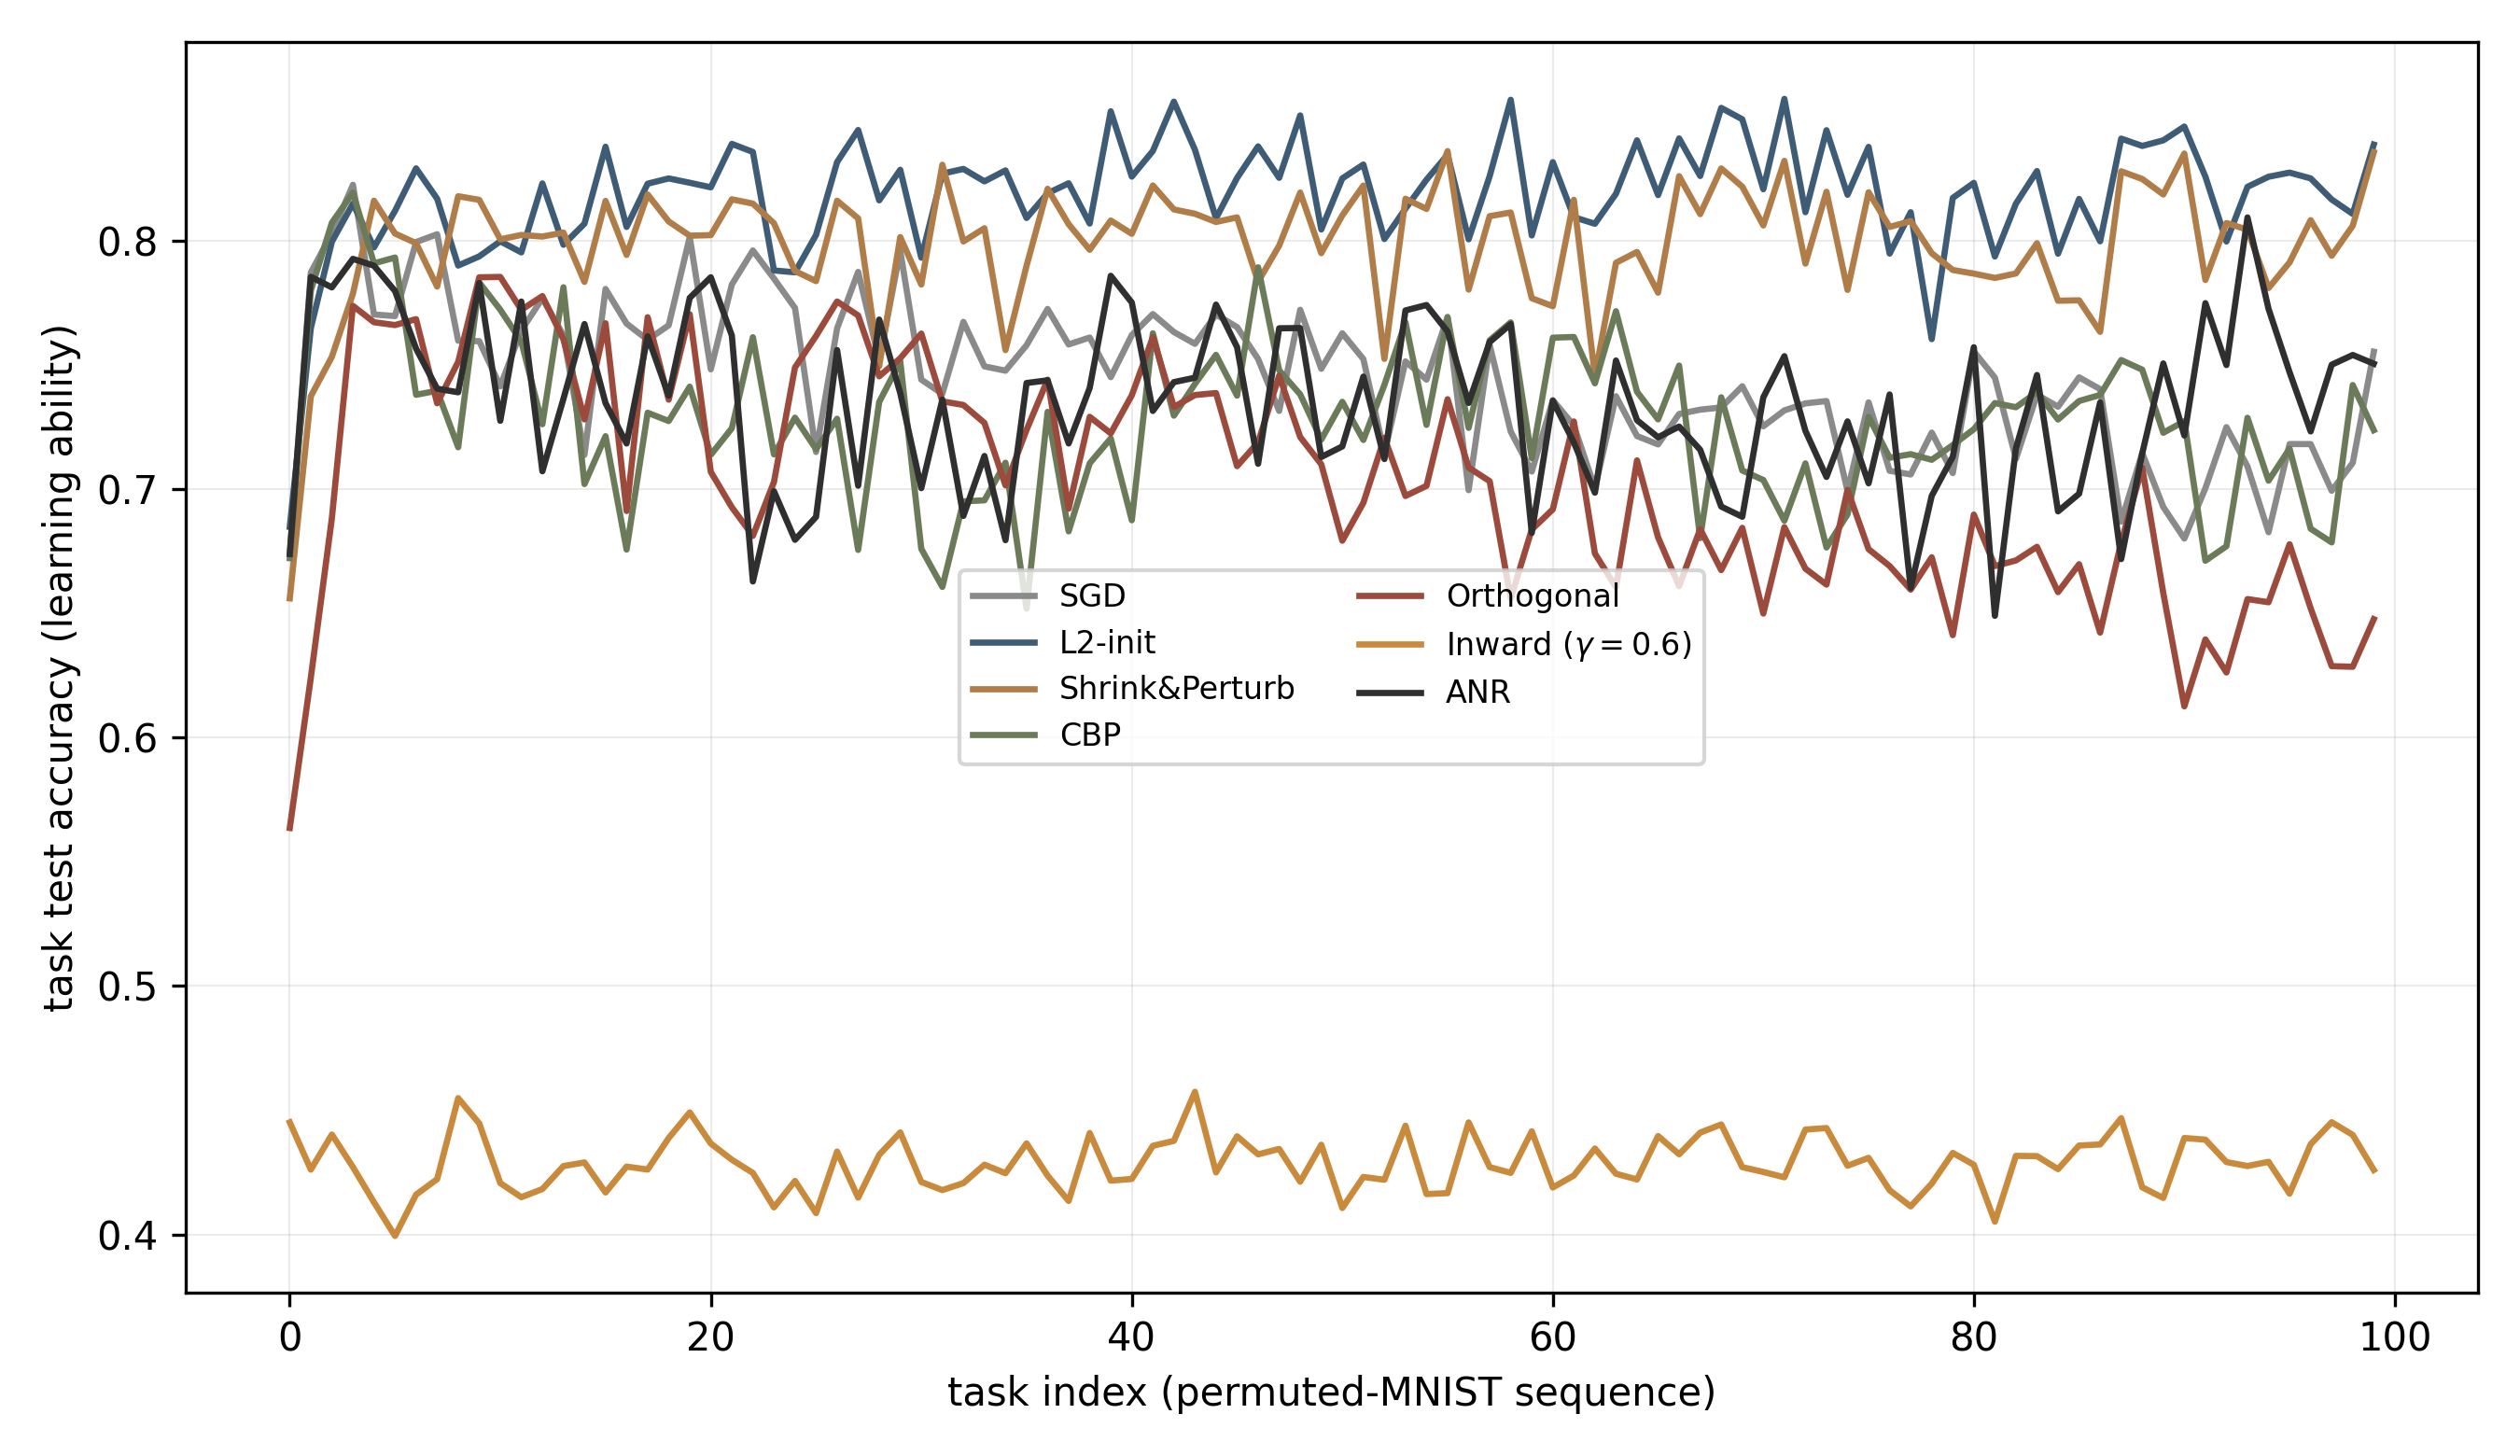
\includegraphics[width=\columnwidth]{figs/plasticity_curves.png}
\caption{Per-task test accuracy over the $100$-task sequence (mean of five seeds).
SGD, CBP, and orthogonal steering decay; the norm-controlled magnitude methods hold
flatter, while inward steering keeps a low norm but at a large accuracy cost
(Cor.~\ref{cor:inward}).}
\label{fig:curves}
\end{figure}

\textbf{Association: decay tracks global-norm growth.} Across the seven arms, the
final global weight norm and plasticity decay are strongly associated
(Pearson $r{=}0.97$, Spearman $\rho{=}0.86$, $n{=}7$ arm-level means); we view this
as an \emph{association} across arms, not a within-run causal estimate. It is robust, and not an outlier artifact: stable across all seeds (per-seed arm-level
$r\in[0.84,0.94]$, mean $0.90$) and to leave-one-arm-out removal ($r\in[0.95,0.98]$;
dropping even the low-norm inward arm gives $0.97$, the high-norm orthogonal arm
$0.95$). We strengthen it by \emph{intervention}: an a-priori geometric sweep of the
L2-init coefficient
$\lambda\in\{0,10^{-3},3{\times}10^{-3},10^{-2},3{\times}10^{-2},10^{-1}\}$ (five
seeds) drives the final norm down monotonically ($20.4\!\to\!4.3$); accuracy peaks at
$\lambda{=}10^{-2}$ ($0.819$) and decay reaches its floor across
$\lambda\!\in\![10^{-2},3\!\times\!10^{-2}]$ (decay $0.047$ then $0.043$; norms $6.6$
then $5.4$), while over-regularization at $\lambda{=}10^{-1}$ worsens both (norm
$4.3$, decay $0.080$, accuracy $0.693$)---a U-shape. As within-family interventional
evidence this is consistent with the cross-arm association but is not definitive
causal proof (gains could arise from regularization effects other than norm
reduction).

\textbf{Directional ablations validate the two regimes.} The matched-step
directional arms behave as Cor.~\ref{cor:orth}--\ref{cor:inward} predict:
\emph{orthogonal steering} attains the largest final norm ($25.1$) and decay
($0.183$), unable to reduce the norm, while \emph{inward steering} drives the norm to
$2.3$ but collapses accuracy to $0.429$. Both have matched-step deviation
{$\le2.2{\times}10^{-7}$}~(Table~\ref{tab:main}), confirming genuine directional---not disguised
magnitude---changes. {A step-wise audit of the orthogonal arm directly confirms
Cor.~\ref{cor:orth}: its updates remain orthogonal to $\theta$ (mean
update--$\theta$ cosine ${-}6{\times}10^{-11}$), so the net rise of squared
global norm matches the accumulated $\sum_t\eta_t^{2}$ within a relative error of
$3{\times}10^{-8}$ (five seeds).}

\textbf{A radial-coefficient sweep resolves the trade-off.} We sweep the inward
radial coefficient $\gamma$ of the inward rule ($\gamma{=}0$ is SGD; larger $\gamma$
allocates more of the fixed-length step inward) over $\{0,0.2,0.4,0.6,0.8,1.0\}$ under
the identical protocol (five seeds; $\gamma{=}0$/$0.6$ reproduce the SGD/inward rows of
Table~\ref{tab:main} exactly). The final norm falls \emph{monotonically}
{across the six settings ($20.4\!\to\!4.1\!\to\!3.1\!\to\!2.3\!\to\!0.25\!\to\!{<}0.05$;
the $\gamma{=}1.0$ norm collapses below the figure's log-axis floor)}, confirming
direction \emph{can} control the
norm (Cor.~\ref{cor:inward}; Fig.~\ref{fig:radial}); accuracy, however, is
non-monotonic---a \emph{mild} bias ($\gamma{=}0.2$) modestly beats SGD ($0.763$ vs.
$0.744$) at norm $4.1$/dormancy $6.2\%$, larger allocations degrade it ($0.655$ at
$0.4$; $0.429$ at $0.6$), and aggressive inward steering collapses learning ($0.157$
at $0.8$; $0.105$ at $1.0$, dormancy $\to100\%$). This makes the radial--tangential
trade-off empirical: inward budget that suppresses the norm is taken from
task descent. Decisively, \emph{no} setting reaches magnitude control---the best
($\gamma{=}0.2$, $0.763$) trails Shrink\&Perturb ($0.799$) and L2-init ($0.819$), and
at matched low norm ($\approx4$) Shrink\&Perturb still wins. Directional norm
control thus offers at most a modest gain over SGD.

\begin{figure}[tb]
\centering
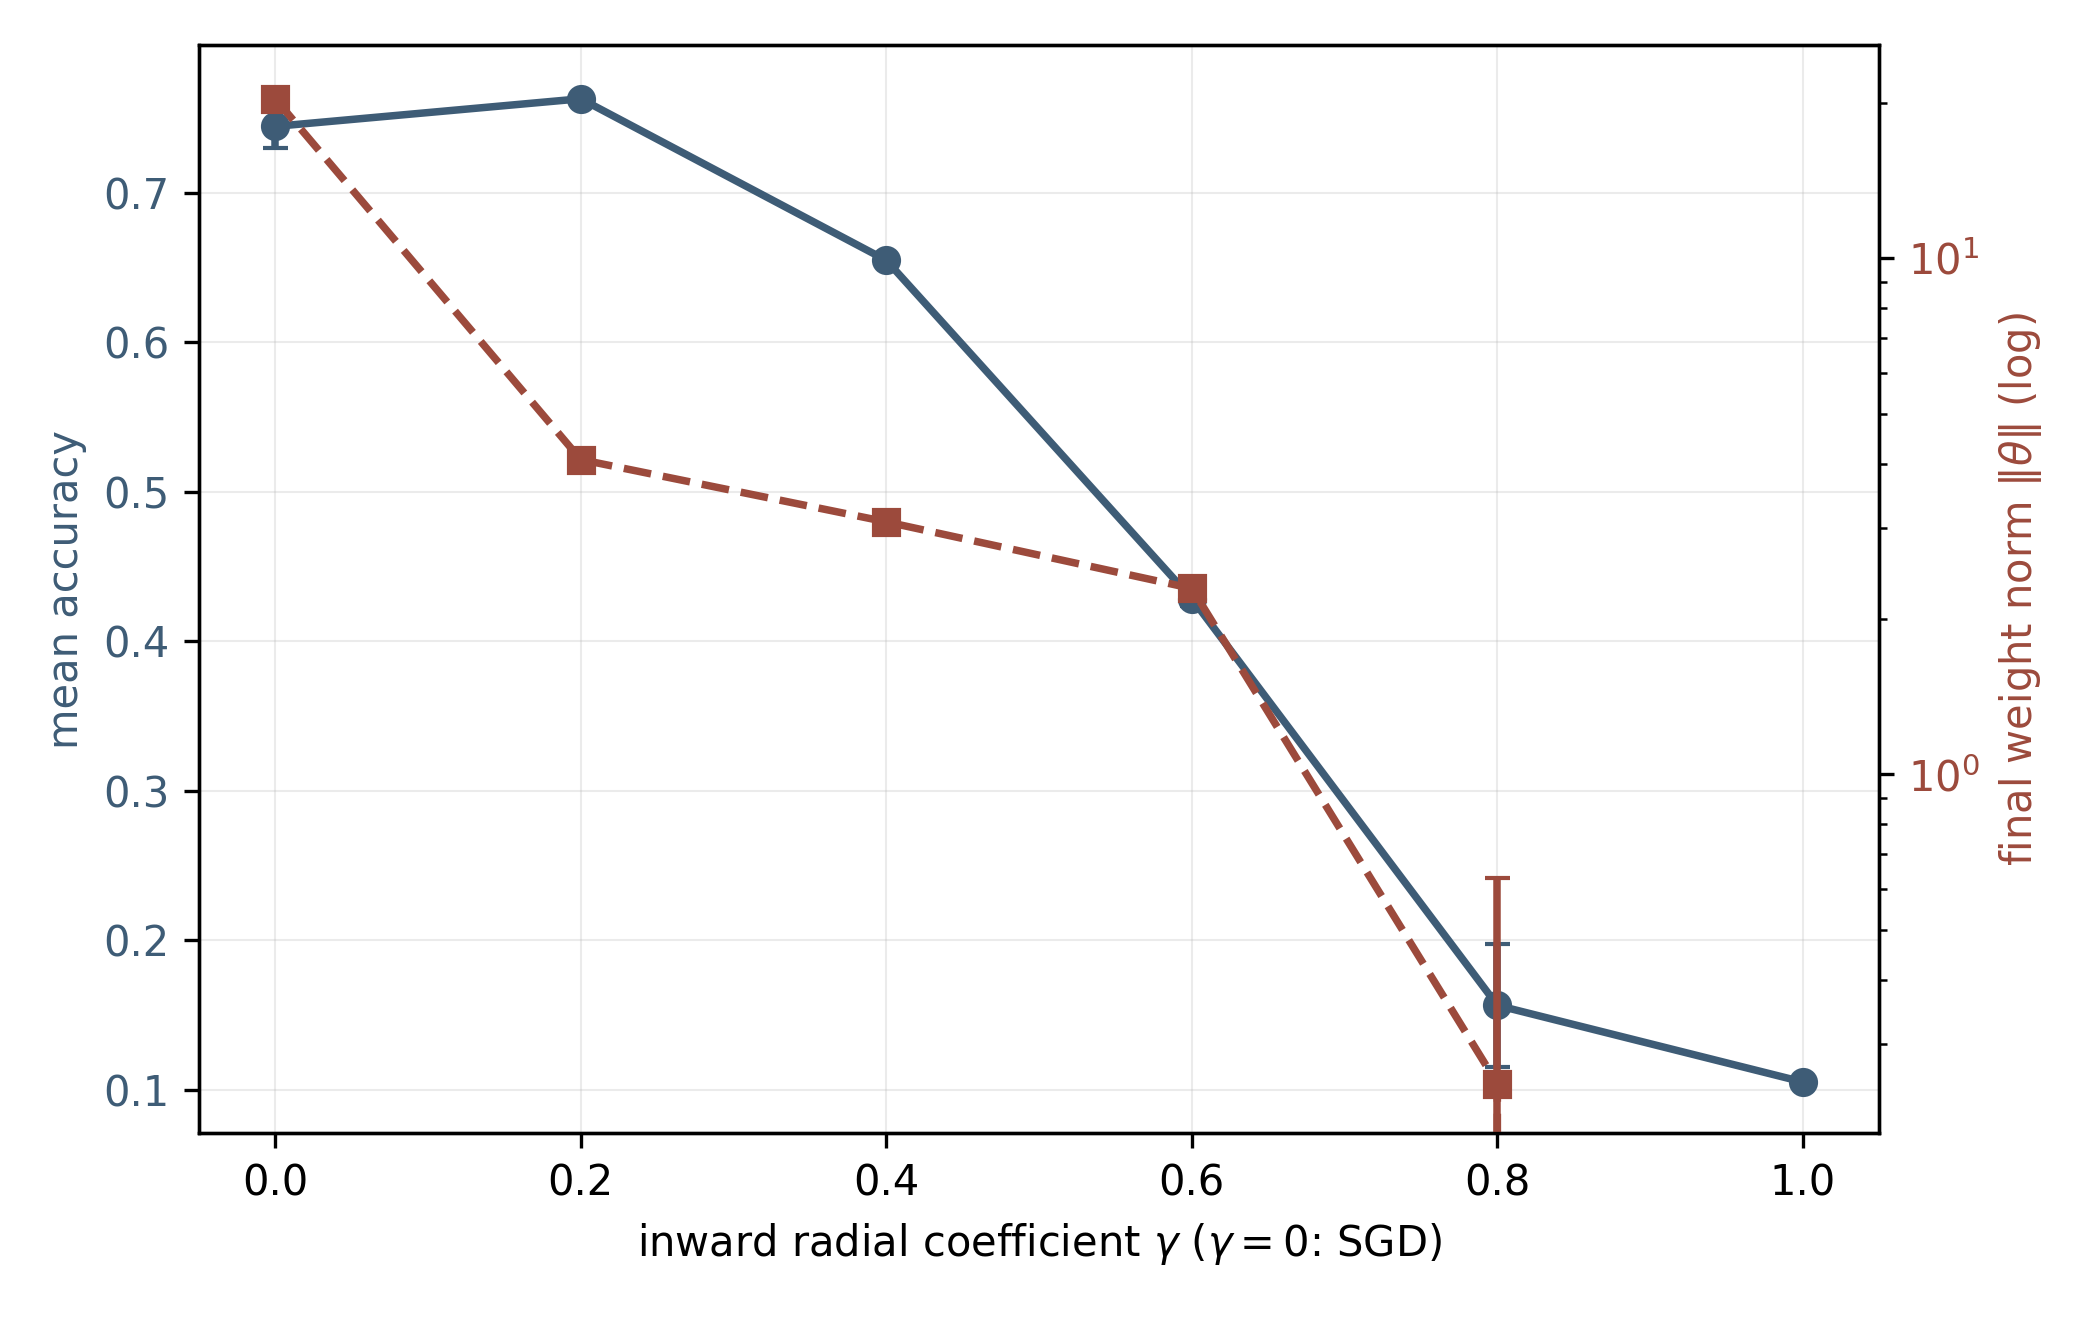
\includegraphics[width=0.92\columnwidth]{figs/radial_sweep.png}
\caption{Radial-coefficient sweep (five seeds, mean$\pm$std; {matched step
$\le2.3{\times}10^{-7}$}). Increasing the inward radial coefficient $\gamma$ monotonically
lowers the final global weight norm (right axis, log) but mean accuracy (left axis)
peaks at a \emph{mild} bias ($\gamma{=}0.2$, above SGD at $\gamma{=}0$) and then it
collapses as aggressive inward steering starves the task-descent budget
($\gamma{\ge}0.8$: dormancy $\to100\%$). No setting reaches magnitude-control
accuracy ($0.799$--$0.819$).}
\label{fig:radial}
\end{figure}

\textbf{Reference magnitude methods preserve plasticity here.} The methods
\emph{allowed} to reduce the global norm---L2-init ($0.819\pm0.003$, decay $0.047$,
norm $6.6$) and Shrink\&Perturb ($0.799\pm0.010$, decay $0.046$, norm $4.2$)---beat
SGD ($0.744$) and every directional arm. Paired across five seeds ($5/5$ in each
comparison): L2-init exceeds SGD by $+0.074$, Shrink\&Perturb exceeds SGD by
$+0.055$, and L2-init exceeds Shrink\&Perturb by $+0.020$; we report paired-seed
differences rather than significance tests given $n{=}5$. The ranking is
metric-dependent (L2-init best accuracy, Shrink\&Perturb marginally lower decay,
$0.046$ vs.\ $0.047$), so neither dominates on every metric---a \emph{regime} result,
not a universal remedy.

\textbf{Effective rank tracks accuracy, weakly relates to decay.} Across arms,
final effective feature rank is associated with mean accuracy
($r{=}0.89$) but only weakly (and negatively) with decay ($r{=}-0.21$). We
therefore view effective rank as a secondary, accuracy-correlated diagnostic, and
do not attribute decay to rank collapse.

\textbf{Adaptive-Norm-Revive: an informative negative.} ANR cuts decay
($0.090$ vs.\ SGD $0.133$) and drives dormancy from $0.212$ to $0.006$, yet reaches
only $0.735\pm0.010$ accuracy---below Shrink\&Perturb on every seed ($-0.064$, $0/5$)
and indistinguishable from SGD ($-0.010$, $2/5$). Targeted per-unit control thus does
\emph{not} beat global shrinking, and eliminating dormancy is by itself insufficient.
A component ablation reveals why: dormant-unit \emph{revival} is the useful element
(revive-only $0.761$, decay $0.072$; the best variant), whereas the per-unit
\emph{shrink} is harmful (shrink-only $0.690$, decay $0.150$, below SGD, dormancy
rising to $0.362$); combining them ($0.735$) is worse than revival alone. Each variant remains below the magnitude methods, so the
per-unit norm cap---not the revival---explains ANR's underperformance.

\textbf{Regime dependence: width and task geometry.} The width-$16$ association is
\emph{not} universal (Table~\ref{tab:regime}). Repeating the seven-arm protocol at
width $64$, degradation is milder (SGD decay $0.052$ vs.\ $0.133$; accuracy
$0.839$), L2-init is again the best arm ($0.856$, decay $0.023$), and the arm-level
norm--decay association also declines to $r{=}0.45$. At width $128$ the stress has
largely abated (SGD decay $0.032$), and the full-rank arms cluster with no
magnitude-control advantage; the association {changes sign} to $r{=}-0.52$.
Changing the task geometry to rotated MNIST---a milder stream in which plain SGD
already retains plasticity (decay $\approx0.02$)---{makes it more strongly
negative}:
$r{=}-0.94$ (width-$16$ MLP) and $r{=}-0.82$ (small CNN), because there the
highest-norm arms {(SGD and, for the MLP, CBP)} rank among the \emph{best} performers. {Negative
values occur only where plain SGD barely loses plasticity (SGD decay ${\le}0.032$,
below the width-$16$ seed std of $0.036$), so we interpret them as the association
vanishing when little plasticity loss remains to explain, not as an opposite
mechanism.} Two readings
follow: the positive norm--decay coupling is a property of the capacity-constrained
\emph{stress} regime, not of continual learning in general; yet in every regime the
\emph{inward}-steering arm still collapses accuracy (e.g.\ $0.618$ at width $64$;
$0.441$ on rotated MNIST) exactly as Cor.~\ref{cor:inward} predicts---so the
geometric result is regime-independent even though the empirical correlation is not.
We thus treat weight-norm growth as a regime-specific \emph{correlate}, not a
universal cause.

\begin{table}[tb]
\caption{Regime dependence: arm-level Pearson $r$ between final global weight norm and plasticity decay (a descriptive statistic across arms, not a seed-level causal estimate; same protocol, CNN differences in Sec.~VI). The strong positive width-16 permuted-MNIST association weakens at width 64 and is absent where plain SGD barely loses plasticity (width 128, rotated MNIST). $h$: hidden width; all MLPs use 784-$h$-$h$-10.}
\label{tab:regime}
\centering
\renewcommand{\arraystretch}{1.05}
\footnotesize
\setlength{\tabcolsep}{5pt}
\begin{tabular}{@{}lcc c r@{}}
\toprule
\textbf{Regime} & \textbf{Seeds} & \textbf{Arms} & {\textbf{SGD decay}} & \textbf{$r$}\\
\midrule
Permuted MNIST, MLP $h{=}16$  & 5 & 7 & {$0.133$} & $+0.97$\\
Permuted MNIST, MLP $h{=}64$  & 5 & 7 & {$0.052$} & $+0.45$\\
Permuted MNIST, MLP $h{=}128$ & 5 & 7 & {$0.032$} & $-0.52$\\
Rotated MNIST, MLP $h{=}16$   & 5 & 7 & {$0.021$} & $-0.94$\\
Rotated MNIST, small CNN      & 3 & 6 & {$0.004$} & $-0.82$\\
\bottomrule
\end{tabular}
\end{table}

\section{Discussion}\label{sec:disc}
The evidence has three levels: a descriptive cross-arm association ($r$=0.97), a within-family intervention (the $\lambda$-sweep) that moves decay with norm-control strength, and a geometric identity (Cors.~1--2) whose predictions the directional arms match exactly. Direction is not irrelevant: inward steering can lower the norm, but only by spending update budget on the radial component, reducing accuracy, while orthogonal steering cannot lower it at all. Since the association weakens with width and is absent where plasticity loss is mild, global-norm growth is a regime-specific correlate, consistent with the multi-cause view [32]: norm growth tracks decay only where it is the dominant stressor.

\textbf{Novelty.} Against prior work linking plasticity to magnitude, initialization
distance, dormant units, and representation collapse, our distinct contribution is the
controlled isolation of update \emph{direction} from \emph{magnitude} via exact
step-size matching, the fixed-step global-norm analysis with its radial--tangential
reading, and the finding that the norm--plasticity coupling is
\emph{regime-dependent}---strong under capacity stress, weaker at width 64, and absent where plasticity loss is mild---rather than a general law.

\textbf{Limitations.} Scope is MNIST-family only (permuted and rotated; no
CIFAR/ImageNet scale) on small two-hidden-layer MLPs plus one small CNN, so larger
and deeper models are untested. {Our Continual Backprop is a simplified
reimplementation (no maturity threshold, untuned $\rho$), so its results should not be
read as representative of tuned Continual Backprop.} We do not study normalized architectures
(BatchNorm/LayerNorm), which rescale activations independently of
$\lVert\theta\rVert$ and alter the geometry of Prop.~\ref{prop:floor}, nor adaptive
optimizers (Adam~\cite{kingma2015adam}/AdamW), whose per-coordinate steps break the
fixed-global-step premise. The norm--decay and rank--accuracy relationships are arm-level associations
($n{=}7$), not seed-level causal estimates (the $\lambda$-sweep adds only one
within-family intervention); the directional interventions are a radial sweep plus an
orthogonal endpoint, not an exhaustive search (e.g.\ learned or subspace directions);
and the proposition concerns the \emph{global} norm, leaving per-layer/per-unit
geometry and non-norm pathologies out of scope. Finally, ANR did not beat global
magnitude control (a better-tuned targeted method might); plasticity is measured only
by per-task accuracy; and compute overhead was not benchmarked (all arms share the
$60$-step/task budget, differing only by a per-step vector operation).

\section{Conclusion}
Under exact step-size matching on a capacity-constrained $100$-task permuted-MNIST
regime (with wider-MLP and rotated-MNIST tests), controlling update \emph{magnitude}
preserves plasticity more effectively than the \emph{directional} interventions we
evaluate. A fixed-step identity shows direction can reduce the global norm only via
an inward radial component drawn from the descent budget, and a radial sweep confirms
the trade-off: inward steering drives the norm down but no setting matches magnitude
control, and strong inward allocation collapses learning. Direction is not
irrelevant---only that fixed-step directional norm control is insufficient for
plasticity here. Critically, the norm--plasticity association is regime-specific
(strong at width $16$, weakening with width and {absent where plasticity loss is
mild width $128$, rotated MNIST}), so weight-norm growth is not a universal
mechanism. Larger
architectures, normalization, adaptive optimizers, and non-norm pathologies remain
the central open questions.

\section*{Reproducibility}
{All code, the frozen configuration, an append-only decision/results log, and a
single-command reproducer will be released upon acceptance. Every number, table row,
and figure comes from the released per-run summaries; step-size matching stays within
tolerance $10^{-4}$ (maximum observed deviation $2.3{\times}10^{-7}$) for every arm.}

\bibliographystyle{IEEEtran}
\bibliography{references}

\end{document}
